\documentclass[11pt,a4paper]{article}

\usepackage[T1]{fontenc}
\usepackage{lmodern}
\usepackage[margin=2.4cm]{geometry}
\usepackage{amsmath,amssymb}
\usepackage{xcolor}
\usepackage{tikz}
\usetikzlibrary{arrows.meta,positioning,shapes.geometric,fit,calc,decorations.pathreplacing,backgrounds}
\usepackage{pgfplots}
\pgfplotsset{compat=1.17}
\usepackage{listings}
\usepackage{booktabs}
\usepackage{tabularx}
\usepackage{caption}
\usepackage{enumitem}
\usepackage[colorlinks=true,linkcolor=blue!60!black,urlcolor=blue!60!black,citecolor=blue!60!black]{hyperref}

% ---------- colours ----------
\definecolor{incol}{HTML}{2E86C1}    % input / word vectors (syn0)
\definecolor{outcol}{HTML}{CA6F1E}   % output vectors (syn1neg / syn1)
\definecolor{poscol}{HTML}{1E8449}   % positive example
\definecolor{negcol}{HTML}{C0392B}   % negative example
\definecolor{codebg}{HTML}{F7F7F7}
\definecolor{notebg}{HTML}{EAF2F8}

% ---------- code listings ----------
\lstdefinestyle{c}{
  language=C,
  basicstyle=\ttfamily\footnotesize,
  keywordstyle=\color{blue!70!black}\bfseries,
  commentstyle=\color{green!45!black}\itshape,
  stringstyle=\color{red!60!black},
  numberstyle=\tiny\color{gray},
  numbers=left,
  numbersep=6pt,
  backgroundcolor=\color{codebg},
  frame=single,
  rulecolor=\color{gray!40},
  breaklines=true,
  columns=fullflexible,
  keepspaces=true,
  showstringspaces=false,
  xleftmargin=1.5em,
  framexleftmargin=1.5em,
  morekeywords={real}
}
\lstset{style=c}

\newcommand{\code}[1]{\texttt{#1}}
\newcommand{\src}[1]{\texttt{word2vec.c:#1}}
\newcommand{\vin}{\mathbf{v}}
\newcommand{\vout}{\mathbf{u}}

% simple shaded "note" box without extra packages
\newsavebox{\notebox}
\newenvironment{note}
  {\par\smallskip\noindent\begin{lrbox}{\notebox}\begin{minipage}{\dimexpr\linewidth-2\fboxsep-2\fboxrule\relax}\small}
  {\end{minipage}\end{lrbox}\fcolorbox{incol!40}{notebg}{\usebox{\notebox}}\par\smallskip}

\title{\textbf{How word2vec Works}\\[4pt]
\large A guided tour of the idea and of the original C implementation}
\author{Notes on \texttt{word2vec.c} and its companion tools}
\date{\today}

\begin{document}
\maketitle

\begin{abstract}
word2vec turns every word of a text corpus into a short, dense vector of real
numbers such that words used in similar contexts end up close together. This
document explains \emph{what} word2vec is trying to achieve, \emph{why} the
training objective produces useful vectors, and \emph{how} the original C program in
this repository (\code{word2vec.c}) implements it: vocabulary building,
subsampling, the sliding context window, the CBOW and skip-gram architectures,
negative sampling, hierarchical softmax, the sigmoid lookup table, the learning-rate
schedule and lock-free multithreading. Line numbers such as \src{450} refer to
the file in this repository. Code listings are excerpts; a few explanatory comments
have been added.
\end{abstract}

\tableofcontents
\newpage

%======================================================================
\section{The goal: meaning as geometry}
%======================================================================

\subsection{The problem with words as symbols}

A computer sees a word as an arbitrary symbol. The simplest numerical encoding is
a \emph{one-hot} vector: with a vocabulary of $V$ words, word $i$ is a vector of
length $V$ with a single~1 at position $i$. One-hot vectors carry no meaning:
every pair of distinct words is equally far apart, so \emph{cat} is as different
from \emph{dog} as it is from \emph{carburettor}.

\subsection{The distributional hypothesis}

word2vec rests on an old idea from linguistics:
\begin{quote}
\emph{``You shall know a word by the company it keeps.''} --- J.\,R.~Firth, 1957
\end{quote}
Words that appear in similar contexts tend to have similar meanings. \emph{Cat}
and \emph{dog} both appear near \emph{pet}, \emph{fed}, \emph{vet} and
\emph{fur}; \emph{carburettor} does not.

\subsection{What word2vec produces}

word2vec learns a mapping
\[
  \text{word } w \;\longmapsto\; \vin_w \in \mathbb{R}^{d}, \qquad d \approx 100\text{--}300 \ll V,
\]
chosen so that words with similar contexts get vectors pointing in similar
directions. Figure~\ref{fig:onehot-vs-dense} contrasts the two representations.

\begin{figure}[ht]
\centering
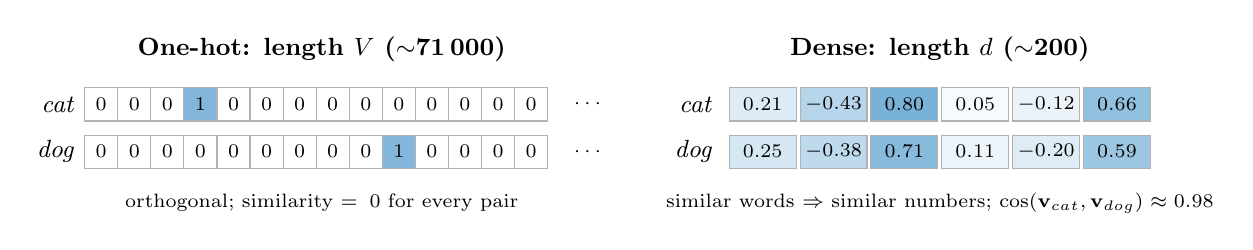
\begin{tikzpicture}[cell/.style={draw=gray!60,minimum size=4.2mm,inner sep=0pt,font=\scriptsize}]
  % one-hot
  \node[anchor=east,font=\small] at (-0.2,0.0) {\emph{cat}};
  \node[anchor=east,font=\small] at (-0.2,-0.6) {\emph{dog}};
  \foreach \i in {0,...,13} {
    \node[cell] at (\i*0.42,0) {0};
    \node[cell] at (\i*0.42,-0.6) {0};
  }
  \node[cell,fill=incol!60] at (3*0.42,0) {1};
  \node[cell,fill=incol!60] at (9*0.42,-0.6) {1};
  \node[font=\scriptsize] at (6.2,0) {$\cdots$};
  \node[font=\scriptsize] at (6.2,-0.6) {$\cdots$};
  \node[font=\small\bfseries] at (2.8,0.7) {One-hot: length $V$ ($\sim$71\,000)};
  \node[font=\scriptsize,text width=6cm,align=center] at (2.8,-1.25) {orthogonal; similarity $=0$ for every pair};

  % dense
  \begin{scope}[xshift=8.4cm]
    \node[anchor=east,font=\small] at (-0.5,0.0) {\emph{cat}};
    \node[anchor=east,font=\small] at (-0.5,-0.6) {\emph{dog}};
    \foreach \v [count=\i from 0] in {0.21,-0.43,0.80,0.05,-0.12,0.66} {
      \pgfmathsetmacro{\shade}{abs(\v)*80}
      \node[cell,minimum width=8.5mm,fill=incol!\shade] at (\i*0.9,0) {$\v$};
    }
    \foreach \v [count=\i from 0] in {0.25,-0.38,0.71,0.11,-0.20,0.59} {
      \pgfmathsetmacro{\shade}{abs(\v)*80}
      \node[cell,minimum width=8.5mm,fill=incol!\shade] at (\i*0.9,-0.6) {$\v$};
    }
    \node[font=\small\bfseries] at (2.25,0.7) {Dense: length $d$ ($\sim$200)};
    \node[font=\scriptsize,text width=7cm,align=center] at (2.25,-1.25) {similar words $\Rightarrow$ similar numbers; $\cos(\vin_{cat},\vin_{dog})\approx 0.98$};
  \end{scope}
\end{tikzpicture}
\caption{One-hot vectors (left) carry no notion of similarity. word2vec's dense vectors (right) put related words close together. The numbers are illustrative.}
\label{fig:onehot-vs-dense}
\end{figure}

The surprising bonus is that the geometry of the space captures \emph{relations},
not only similarity. Differences between vectors encode consistent directions,
so simple vector arithmetic solves analogies:
\[
  \vin_{\text{king}} - \vin_{\text{man}} + \vin_{\text{woman}} \;\approx\; \vin_{\text{queen}}.
\]

\begin{figure}[ht]
\centering
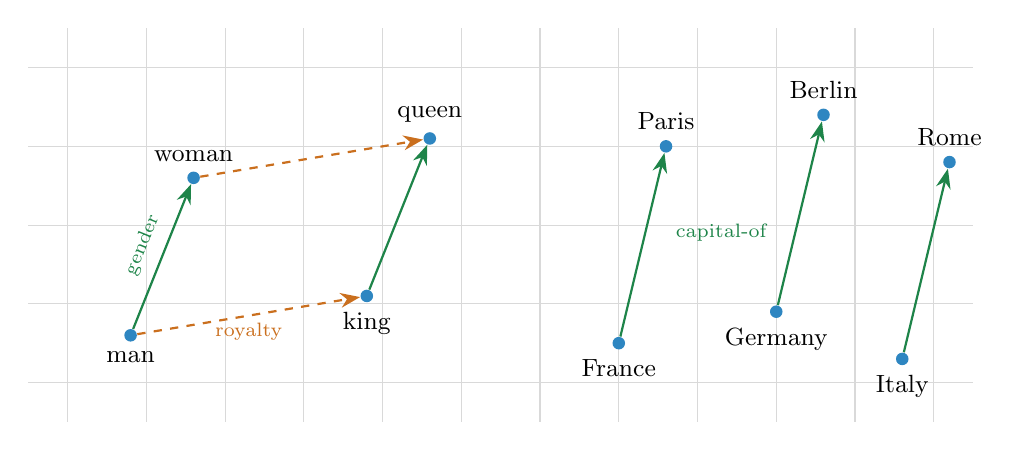
\begin{tikzpicture}[scale=1.0,
    w/.style={circle,fill=incol,inner sep=1.6pt},
    lbl/.style={font=\small}]
  \draw[gray!30,step=1] (-0.5,-0.5) grid (11.5,4.5);
  % gender analogy
  \node[w,label={[lbl]below:man}]   (man)   at (0.8,0.6) {};
  \node[w,label={[lbl]above:woman}] (woman) at (1.6,2.6) {};
  \node[w,label={[lbl]below:king}]  (king)  at (3.8,1.1) {};
  \node[w,label={[lbl]above:queen}] (queen) at (4.6,3.1) {};
  \draw[-{Stealth[length=2.5mm]},thick,poscol] (man) -- (woman);
  \draw[-{Stealth[length=2.5mm]},thick,poscol] (king) -- (queen);
  \draw[-{Stealth[length=2.5mm]},thick,dashed,outcol] (man) -- (king);
  \draw[-{Stealth[length=2.5mm]},thick,dashed,outcol] (woman) -- (queen);
  \node[font=\scriptsize,poscol,rotate=68] at (0.95,1.75) {gender};
  \node[font=\scriptsize,outcol] at (2.3,0.65) {royalty};
  % country-capital analogy
  \node[w,label={[lbl]below:France}]  (fr) at (7.0,0.5) {};
  \node[w,label={[lbl]above:Paris}]   (pa) at (7.6,3.0) {};
  \node[w,label={[lbl]below:Germany}] (de) at (9.0,0.9) {};
  \node[w,label={[lbl]above:Berlin}]  (be) at (9.6,3.4) {};
  \node[w,label={[lbl]below:Italy}]   (it) at (10.6,0.3) {};
  \node[w,label={[lbl]above:Rome}]    (ro) at (11.2,2.8) {};
  \foreach \a/\b in {fr/pa,de/be,it/ro}
    \draw[-{Stealth[length=2.5mm]},thick,poscol] (\a) -- (\b);
  \node[font=\scriptsize,poscol,align=center] at (8.3,1.9) {capital-of};
\end{tikzpicture}
\caption{A 2-D cartoon of the learned space. Consistent relationships become
roughly parallel offsets, which is why \code{word-analogy} can answer
``\emph{man} is to \emph{king} as \emph{woman} is to \underline{\quad}''
by computing $\vin_{king}-\vin_{man}+\vin_{woman}$.}
\label{fig:analogy}
\end{figure}

\subsection{The trick: a fake task}

Nobody tells word2vec what words mean. Instead it trains a tiny neural network
on a \emph{fake prediction task} that can be generated automatically from raw
text: \emph{given a word, predict the words around it} (or the reverse). The
prediction itself is thrown away. The useful product is the network's first
weight matrix, whose rows are the word vectors. To predict contexts well, the
network must give words with similar contexts similar vectors, which is exactly
what we wanted.

%======================================================================
\section{The big picture: from text file to vectors}
%======================================================================

The repository contains five programs. \code{word2vec} does the training; the
others prepare input or use the output (Figure~\ref{fig:pipeline}).

\begin{figure}[ht]
\centering
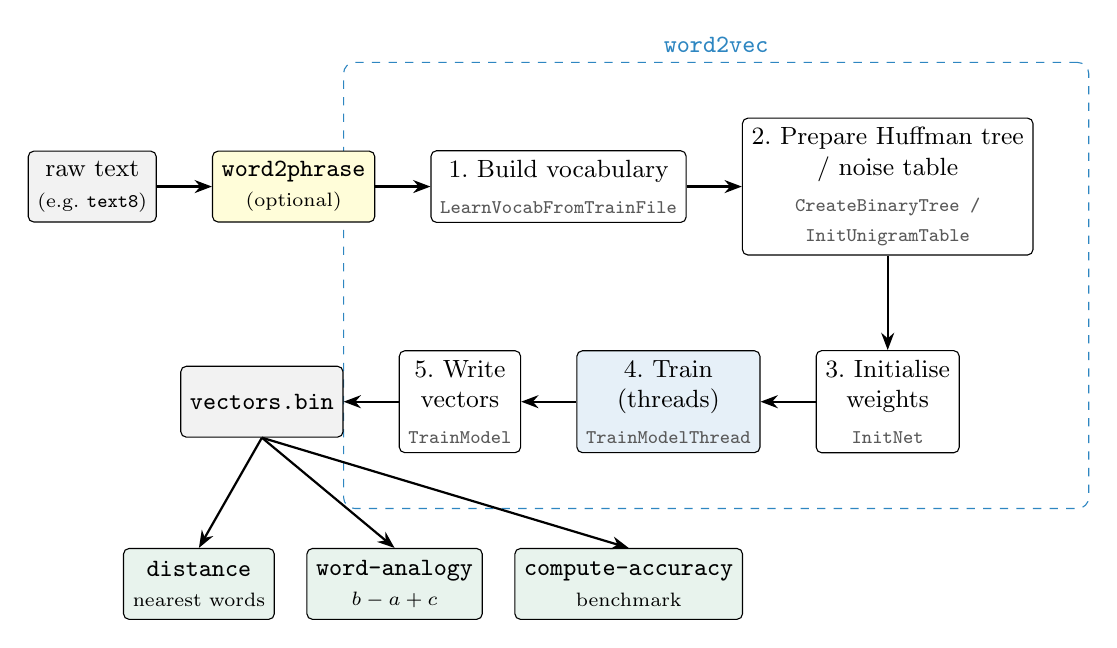
\begin{tikzpicture}[
  node distance=5mm and 7mm,
  box/.style={draw,rounded corners=2pt,align=center,font=\small,minimum height=9mm,fill=white},
  fn/.style={font=\scriptsize\ttfamily,text=gray!70!black},
  arr/.style={-{Stealth[length=2.2mm]},thick}]
  \node[box,fill=gray!10] (corpus) {raw text\\\scriptsize(e.g.\ \code{text8})};
  \node[box,right=of corpus,fill=yellow!15] (phrase) {\code{word2phrase}\\\scriptsize(optional)};
  \node[box,right=of phrase] (vocab) {1.~Build vocabulary\\[2pt]{\scriptsize\ttfamily\color{gray!70!black} LearnVocabFromTrainFile}};
  \node[box,right=of vocab] (prep) {2.~Prepare Huffman tree\\/ noise table\\[2pt]{\scriptsize\ttfamily\color{gray!70!black} CreateBinaryTree /}\\{\scriptsize\ttfamily\color{gray!70!black} InitUnigramTable}};
  \node[box,below=12mm of prep] (init) {3.~Initialise\\weights\\[2pt]{\scriptsize\ttfamily\color{gray!70!black} InitNet}};
  \node[box,left=of init,fill=incol!12] (train) {4.~Train\\(threads)\\[2pt]{\scriptsize\ttfamily\color{gray!70!black} TrainModelThread}};
  \node[box,left=of train] (save) {5.~Write\\vectors\\[2pt]{\scriptsize\ttfamily\color{gray!70!black} TrainModel}};
  \node[box,left=of save,fill=gray!10] (vec) {\code{vectors.bin}};


  \draw[arr] (corpus) -- (phrase);
  \draw[arr] (phrase) -- (vocab);
  \draw[arr] (vocab) -- (prep);
  \draw[arr] (prep) -- (init);
  \draw[arr] (init) -- (train);
  \draw[arr] (train) -- (save);
  \draw[arr] (save) -- (vec);

  \node[box,below=14mm of vec,xshift=-8mm,fill=poscol!10] (dist) {\code{distance}\\\scriptsize nearest words};
  \node[box,right=4mm of dist,fill=poscol!10] (ana) {\code{word-analogy}\\\scriptsize $b-a+c$};
  \node[box,right=4mm of ana,fill=poscol!10] (acc) {\code{compute-accuracy}\\\scriptsize benchmark};
  \draw[arr] (vec.south) -- (dist.north);
  \draw[arr] (vec.south) -- (ana.north);
  \draw[arr] (vec.south) -- (acc.north);

  \begin{scope}[on background layer]
    \node[draw=incol,dashed,rounded corners,fit=(vocab)(prep)(init)(train)(save),inner sep=7mm,
          label={[font=\small\bfseries,incol]above:\code{word2vec}}] {};
  \end{scope}
\end{tikzpicture}
\caption{Overall data flow. Everything inside the dashed box happens in \code{word2vec.c},
driven by \code{TrainModel()} (\src{572}).}
\label{fig:pipeline}
\end{figure}

\code{TrainModel()} is short enough to read in full; it is the outline of the whole
program:

\begin{lstlisting}[firstnumber=579]
  starting_alpha = alpha;
  if (read_vocab_file[0] != 0) ReadVocab(); else LearnVocabFromTrainFile();
  if (save_vocab_file[0] != 0) SaveVocab();
  if (output_file[0] == 0) return;
  InitNet();
  if (negative > 0) InitUnigramTable();
  start = clock();
  for (a = 0; a < num_threads; a++) pthread_create(&pt[a], NULL, TrainModelThread, (void *)a);
  for (a = 0; a < num_threads; a++) pthread_join(pt[a], NULL);
\end{lstlisting}

The rest of this document follows these steps in order.

%======================================================================
\section{Step 1: building the vocabulary}
%======================================================================

\subsection{Tokenising}

\code{ReadWord()} (\src{77}) splits the file on spaces, tabs and newlines. There is
no other preprocessing: punctuation and case are kept as they are, so the corpus is
normally cleaned beforehand. Every newline is turned into the special token
\code{</s>}, which marks a sentence boundary and always sits at vocabulary index~0.

\subsection{Counting with a hash table}

\code{LearnVocabFromTrainFile()} (\src{279}) streams through the corpus once,
counting every word. Lookups use an open-addressing hash table
(\code{vocab\_hash}, 30 million slots) with linear probing:

\begin{lstlisting}[firstnumber=104]
int GetWordHash(char *word) {
  unsigned long long a, hash = 0;
  for (a = 0; a < strlen(word); a++) hash = hash * 257 + word[a];
  hash = hash % vocab_hash_size;
  return hash;
}
\end{lstlisting}

If the table becomes 70\% full, \code{ReduceVocab()} (\src{191}) throws away
all words seen at most \code{min\_reduce} times and increments \code{min\_reduce},
so huge corpora still fit in memory.

\subsection{Sorting and pruning}

\code{SortVocab()} (\src{161}) sorts words by descending count (keeping
\code{</s>} first) and discards words seen fewer than \code{-min-count} times
(default 5). Rare words have too few contexts to learn a good vector, and dropping
them shrinks the model a lot. After sorting, \emph{a word's index is its frequency
rank}; several later steps rely on this.

Each entry is a \code{struct vocab\_word}:

\begin{lstlisting}[firstnumber=37]
struct vocab_word {
  long long cn;          // count in the corpus
  int *point;            // Huffman path: inner-node indices (hierarchical softmax)
  char *word, *code, codelen;  // the string; Huffman code bits and their number
};
\end{lstlisting}

%======================================================================
\section{The model: two matrices and a dot product}
%======================================================================

\subsection{The parameters}

Despite the ``neural network'' label, word2vec's model is simply two
$V\times d$ matrices of floats, where $d$ is \code{layer1\_size} (\code{-size}):

\begin{center}
\begin{tabularx}{\linewidth}{@{}llX@{}}
\toprule
Array & Symbol & Role \\
\midrule
\code{syn0}    & $\vin_w$ & \textbf{input vectors}: the word vectors written to the output file \\
\code{syn1neg} & $\vout_w$ & output vectors used by negative sampling \\
\code{syn1}    & $\vout_n$ & output vectors of the inner nodes of the Huffman tree (hierarchical softmax) \\
\bottomrule
\end{tabularx}
\end{center}

All are stored as flat row-major arrays, so the vector of word $w$ starts at
offset \code{w * layer1\_size}. That is why the training loop is full of
\code{l1 = last\_word * layer1\_size} and \code{l2 = target * layer1\_size}.

\begin{figure}[ht]
\centering
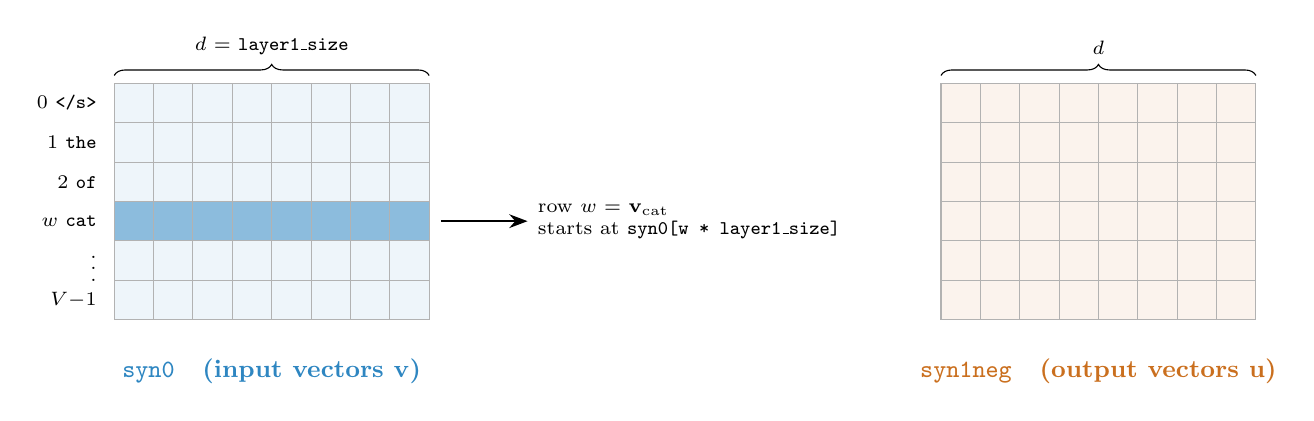
\begin{tikzpicture}[x=5mm,y=5mm]
  \foreach \r in {0,...,5} {
    \foreach \c in {0,...,7} {
      \pgfmathsetmacro{\s}{\r==3 ? 55 : 8}
      \fill[incol!\s] (\c,-\r) rectangle ++(1,-1);
    }
  }
  \draw[gray!60,step=1] (0,0) grid (8,-6);
  \node[anchor=east,font=\scriptsize] at (-0.2,-0.5) {0 \code{</s>}};
  \node[anchor=east,font=\scriptsize] at (-0.2,-1.5) {1 \code{the}};
  \node[anchor=east,font=\scriptsize] at (-0.2,-2.5) {2 \code{of}};
  \node[anchor=east,font=\scriptsize] at (-0.2,-3.5) {$w$ \code{cat}};
  \node[anchor=east,font=\scriptsize] at (-0.2,-4.5) {$\vdots$};
  \node[anchor=east,font=\scriptsize] at (-0.2,-5.5) {$V{-}1$};
  \draw[decorate,decoration={brace,amplitude=4pt}] (0,0.2) -- (8,0.2)
     node[midway,above=4pt,font=\scriptsize] {$d$ = \code{layer1\_size}};
  \node[font=\small\bfseries,incol] at (4,-7.3) {\code{syn0} \; (input vectors $\vin$)};
  \draw[-{Stealth},thick] (8.3,-3.5) -- (10.5,-3.5) node[right,font=\scriptsize,align=left]
     {row $w$ = $\vin_{\text{cat}}$\\starts at \code{syn0[w * layer1\_size]}};

  \begin{scope}[xshift=105mm]
  \foreach \r in {0,...,5} {
    \foreach \c in {0,...,7} {
      \fill[outcol!8] (\c,-\r) rectangle ++(1,-1);
    }
  }
  \draw[gray!60,step=1] (0,0) grid (8,-6);
  \node[font=\small\bfseries,outcol] at (4,-7.3) {\code{syn1neg} \; (output vectors $\vout$)};
  \draw[decorate,decoration={brace,amplitude=4pt}] (0,0.2) -- (8,0.2)
     node[midway,above=4pt,font=\scriptsize] {$d$};
  \end{scope}
\end{tikzpicture}
\caption{Memory layout of the two weight matrices. Every word has \emph{two}
vectors: one used when it is the input, one used when it is the prediction target.
Only \code{syn0} is saved.}
\end{figure}

\subsection{Initialisation}

\code{InitNet()} (\src{361}) fills \code{syn0} with small random numbers,
uniform in $[-\tfrac{0.5}{d},\,\tfrac{0.5}{d}]$, and sets the output matrices to
zero:

\begin{lstlisting}[firstnumber=378]
  for (a = 0; a < vocab_size; a++) for (b = 0; b < layer1_size; b++) {
    next_random = next_random * (unsigned long long)25214903917 + 11;
    syn0[a * layer1_size + b] = (((next_random & 0xFFFF) / (real)65536) - 0.5) / layer1_size;
  }
\end{lstlisting}

The expression \code{next\_random * 25214903917 + 11} is a linear congruential
random-number generator. It appears throughout the code because it is much
faster than calling \code{rand()}.

\subsection{The score}

The model's only computation is a dot product. The score for ``word $o$ appears
in the context of word $c$'' is
\[
  s(c,o) = \vin_c^{\top}\vout_o ,
\]
turned into a probability with the logistic sigmoid
$\sigma(x) = 1/(1+e^{-x})$. High dot product means ``likely neighbours''.

%======================================================================
\section{Step 4a: generating training examples}
%======================================================================

Each training thread runs \code{TrainModelThread()} (\src{385}). Its outer loop
reads one ``sentence'' at a time (up to the next \code{</s>}, at most 1000 words)
into the array \code{sen[]}, then slides over it word by word.

\subsection{Subsampling frequent words}

Very frequent words such as \emph{the}, \emph{of} and \emph{a} appear in nearly
every context and so carry little information. They also dominate training time.
While reading a sentence, the code randomly drops each occurrence of word $w$:

\begin{lstlisting}[firstnumber=423]
        if (sample > 0) {
          real ran = (sqrt(vocab[word].cn / (sample * train_words)) + 1) * (sample * train_words) / vocab[word].cn;
          next_random = next_random * (unsigned long long)25214903917 + 11;
          if (ran < (next_random & 0xFFFF) / (real)65536) continue;
        }
\end{lstlisting}

Writing $f(w) = \code{cn}/\code{train\_words}$ for the word's relative frequency and
$t$ for \code{-sample}, the probability of \emph{keeping} an occurrence is
\[
  P_{\text{keep}}(w) = \left(\sqrt{\frac{f(w)}{t}} + 1\right)\frac{t}{f(w)} .
\]
Words with $f(w)$ below about $2.6\,t$ have $P_{\text{keep}}\ge 1$ and are always kept;
frequent words are aggressively thinned (Figure~\ref{fig:subsample}). Dropping words
also effectively \emph{widens} the context window, since the surviving neighbours
were originally further apart.

\begin{figure}[ht]
\centering
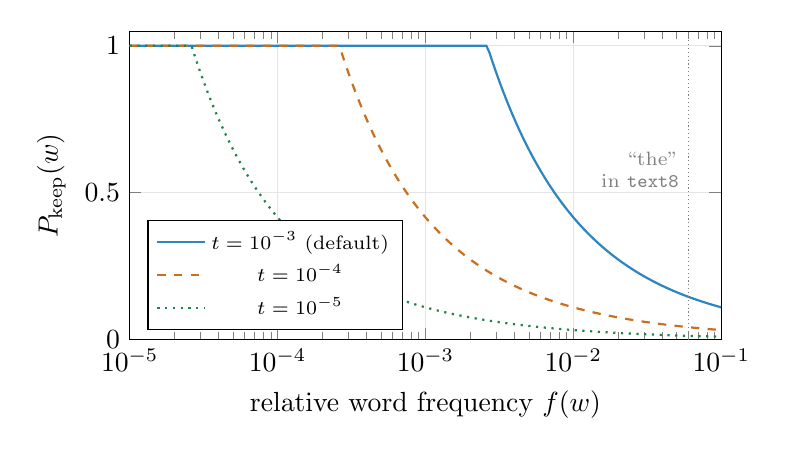
\begin{tikzpicture}
\begin{axis}[
  width=0.75\linewidth,height=5.5cm,
  xmode=log,
  xlabel={relative word frequency $f(w)$},
  ylabel={$P_{\text{keep}}(w)$},
  ymin=0,ymax=1.05,xmin=1e-5,xmax=1e-1,
  grid=major,grid style={gray!20},
  legend pos=south west,legend style={font=\scriptsize},
  every axis plot/.append style={thick,samples=200,domain=1e-5:1e-1}]
  \addplot[incol] {min(1,(sqrt(x/1e-3)+1)*1e-3/x)};
  \addplot[outcol,dashed] {min(1,(sqrt(x/1e-4)+1)*1e-4/x)};
  \addplot[poscol,dotted] {min(1,(sqrt(x/1e-5)+1)*1e-5/x)};
  \legend{{$t=10^{-3}$ (default)},{$t=10^{-4}$},{$t=10^{-5}$}}
  \draw[gray,densely dotted] (axis cs:0.06,0) -- (axis cs:0.06,1.05)
     node[pos=0.55,left,font=\scriptsize,align=right] {``the''\\in \code{text8}};
\end{axis}
\end{tikzpicture}
\caption{Probability that an occurrence survives subsampling. Rare words are always
kept; with $t=10^{-4}$ only about 4\% of the occurrences of \emph{the} survive.}
\label{fig:subsample}
\end{figure}

\subsection{The sliding context window}

For every position in the sentence, the current word \code{word} is the
\emph{centre}. Its context is the words up to \code{window} positions to the left and
right. The code first draws a random shrink amount \code{b} in $[0,\,\code{window}-1]$,
so the effective window size is $\code{window}-b$, uniformly between 1 and
\code{window}:

\begin{lstlisting}[firstnumber=448]
    next_random = next_random * (unsigned long long)25214903917 + 11;
    b = next_random % window;
\end{lstlisting}

\begin{lstlisting}[firstnumber=453]
      for (a = b; a < window * 2 + 1 - b; a++) if (a != window) {
        c = sentence_position - window + a;   // index of a context word
\end{lstlisting}

This is a cheap way to give near neighbours more weight: a word at distance 1 is
always inside the window, a word at distance \code{window} only $1/\code{window}$ of
the time.

\begin{figure}[ht]
\centering
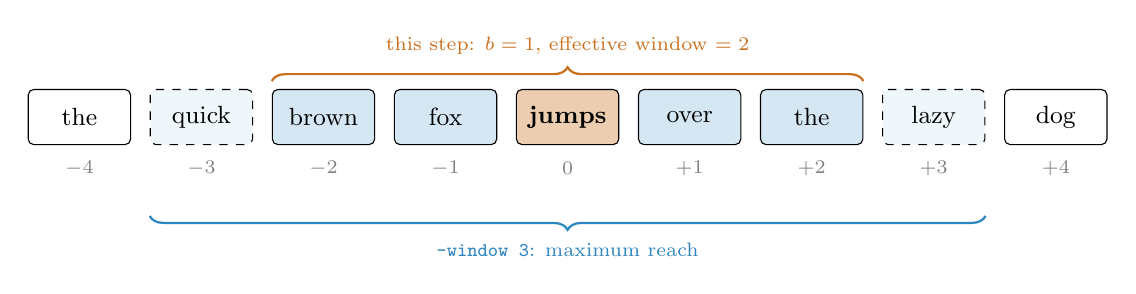
\begin{tikzpicture}[
  tok/.style={draw,rounded corners=2pt,minimum height=7mm,minimum width=13mm,font=\small},
  ctx/.style={tok,fill=incol!20},
  cen/.style={tok,fill=outcol!35,font=\small\bfseries},
  far/.style={tok,fill=incol!7,dashed}]
  \node[tok] (w0) at (0,0) {the};
  \node[far] (w1) at (1.55,0) {quick};
  \node[ctx] (w2) at (3.1,0) {brown};
  \node[ctx] (w3) at (4.65,0) {fox};
  \node[cen] (w4) at (6.2,0) {jumps};
  \node[ctx] (w5) at (7.75,0) {over};
  \node[ctx] (w6) at (9.3,0) {the};
  \node[far] (w7) at (10.85,0) {lazy};
  \node[tok] (w8) at (12.4,0) {dog};
  \foreach \i/\o in {0/-4,1/-3,2/-2,3/-1,4/0,5/+1,6/+2,7/+3,8/+4}
    \node[font=\scriptsize,gray] at ($(w\i)+(0,-0.65)$) {$\o$};
  \draw[decorate,decoration={brace,amplitude=5pt,mirror},thick,incol]
     ($(w1.south west)+(0,-0.9)$) -- ($(w7.south east)+(0,-0.9)$)
     node[midway,below=6pt,font=\scriptsize] {\code{-window 3}: maximum reach};
  \draw[decorate,decoration={brace,amplitude=5pt},thick,outcol]
     ($(w2.north west)+(0,0.1)$) -- ($(w6.north east)+(0,0.1)$)
     node[midway,above=6pt,font=\scriptsize] {this step: $b=1$, effective window $=2$};
\end{tikzpicture}
\caption{The context window around the centre word \emph{jumps} (at
\code{sentence\_position}). Solid blue words are used in this step; dashed ones are
inside the maximum window but cut by the random shrink $b$.}
\label{fig:window}
\end{figure}

%======================================================================
\section{Step 4b: the two architectures}
%======================================================================

The \code{-cbow} flag chooses how the centre word and its context are turned into
predictions (Figure~\ref{fig:archs}).

\begin{figure}[ht]
\centering
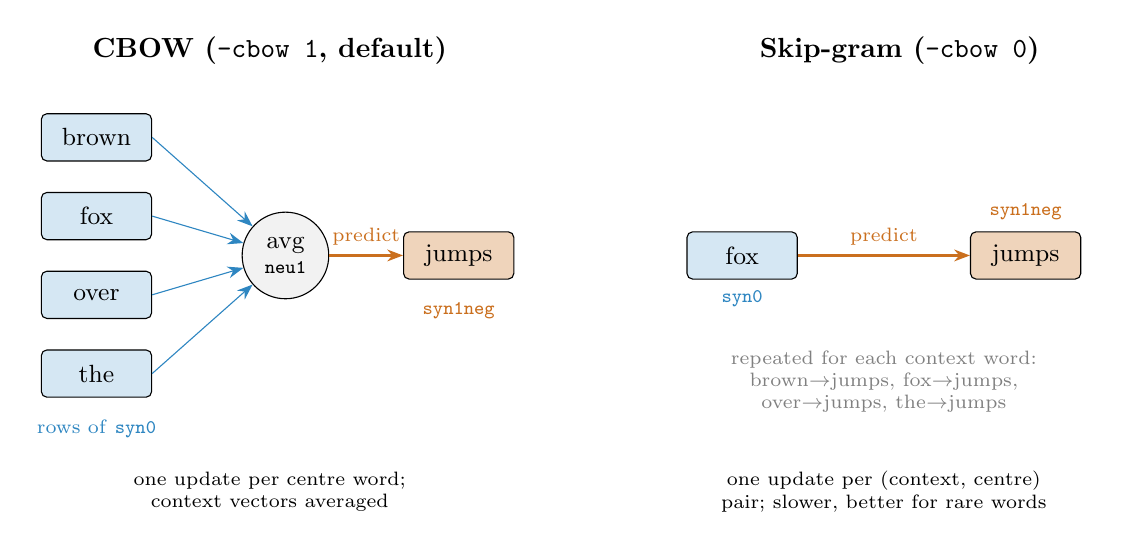
\begin{tikzpicture}[
  wn/.style={draw,rounded corners=2pt,minimum width=14mm,minimum height=6mm,font=\small},
  inw/.style={wn,fill=incol!20},
  outw/.style={wn,fill=outcol!30},
  hid/.style={draw,circle,minimum size=11mm,font=\small,fill=gray!10},
  arr/.style={-{Stealth[length=2mm]}}]
  % ---- CBOW ----
  \node[font=\bfseries] at (2.2,2.6) {CBOW (\code{-cbow 1}, default)};
  \node[inw] (c1) at (0,1.5)  {brown};
  \node[inw] (c2) at (0,0.5)  {fox};
  \node[inw] (c3) at (0,-0.5) {over};
  \node[inw] (c4) at (0,-1.5) {the};
  \node[hid,align=center] (h) at (2.4,0) {avg\\[-2pt]\scriptsize\code{neu1}};
  \node[outw] (o) at (4.6,0) {jumps};
  \foreach \i in {1,...,4} \draw[arr,incol] (c\i.east) -- (h);
  \draw[arr,outcol,thick] (h) -- (o) node[midway,above,font=\scriptsize] {predict};
  \node[font=\scriptsize,incol] at (0,-2.2) {rows of \code{syn0}};
  \node[font=\scriptsize,outcol] at (4.6,-0.7) {\code{syn1neg}};
  \node[font=\scriptsize,text width=5.5cm,align=center] at (2.2,-3.0)
     {one update per centre word; context vectors averaged};

  % ---- Skip-gram ----
  \begin{scope}[xshift=8.2cm]
  \node[font=\bfseries] at (2.0,2.6) {Skip-gram (\code{-cbow 0})};
  \node[inw] (s) at (0,0) {fox};
  \node[outw] (t) at (3.6,0) {jumps};
  \draw[arr,outcol,thick] (s) -- (t) node[midway,above,font=\scriptsize] {predict};
  \node[font=\scriptsize,gray,text width=4.5cm,align=center] at (1.8,-1.6)
     {repeated for each context word:\\ brown$\to$jumps, fox$\to$jumps,\\ over$\to$jumps, the$\to$jumps};
  \node[font=\scriptsize,incol] at (0,-0.55) {\code{syn0}};
  \node[font=\scriptsize,outcol] at (3.6,0.55) {\code{syn1neg}};
  \node[font=\scriptsize,text width=5.5cm,align=center] at (1.8,-3.0)
     {one update per (context, centre) pair; slower, better for rare words};
  \end{scope}
\end{tikzpicture}
\caption{The two architectures for the window of Figure~\ref{fig:window}. Blue boxes
are looked up in \code{syn0}; the orange box is the prediction target, scored with
\code{syn1neg} (or \code{syn1}).}
\label{fig:archs}
\end{figure}

\subsection{CBOW: continuous bag of words}

CBOW predicts the centre word from its context. The context vectors are
\emph{averaged} into a hidden vector $\mathbf{h}$ (\code{neu1}). Word order inside
the window is ignored, hence ``bag of words'':
\[
  \mathbf{h} = \frac{1}{|C|}\sum_{c\in C}\vin_c .
\]
\begin{lstlisting}[firstnumber=459]
        for (c = 0; c < layer1_size; c++) neu1[c] += syn0[c + last_word * layer1_size];
        cw++;
      }
      if (cw) {
        for (c = 0; c < layer1_size; c++) neu1[c] /= cw;
\end{lstlisting}
$\mathbf{h}$ is then scored against the centre word's output vector. The resulting
error vector \code{neu1e} is added, \emph{undivided}, to every context word's input
vector (\src{501--508}).

\subsection{Skip-gram}

Skip-gram does one prediction per (context word, centre word) pair. The paper
describes it as ``predict each context word from the centre word''. The code does the
mirror image: it uses the \emph{context} word's input vector (\code{l1 = last\_word
* layer1\_size}) to predict the \emph{centre} word (\code{word}) at the output.
Because every pair is visited both ways as the window slides, the two formulations
see the same set of pairs.

\begin{lstlisting}[firstnumber=511]
      for (a = b; a < window * 2 + 1 - b; a++) if (a != window) {
        ...
        last_word = sen[c];
        l1 = last_word * layer1_size;   // input: context word
        for (c = 0; c < layer1_size; c++) neu1e[c] = 0;
        // ... score syn0[l1] against the centre word 'word' ...
        for (c = 0; c < layer1_size; c++) syn0[c + l1] += neu1e[c];
      }
\end{lstlisting}

In both cases the remaining question is: \emph{how do we turn ``this input should
predict that word'' into a gradient cheaply?}

%======================================================================
\section{Step 4c: making the output layer cheap}
%======================================================================

The textbook objective is a softmax over the whole vocabulary:
\[
  p(o \mid c) = \frac{\exp(\vin_c^{\top}\vout_o)}{\sum_{w=1}^{V}\exp(\vin_c^{\top}\vout_w)} .
\]
The denominator touches all $V$ output vectors, roughly 71\,000 dot products for
\code{text8} and millions for large corpora, \emph{for every single training pair}.
word2vec offers two approximations that cost $O(k)$ or $O(\log V)$ instead.
They can be used together, but normally one is chosen: \code{-negative 5 -hs 0}
(the default) or \code{-negative 0 -hs 1}.

\subsection{Negative sampling (\texttt{-negative k})}

Negative sampling replaces the $V$-way classification with $k+1$ independent
yes/no questions: ``is this pair a real (context, word) pair from the corpus, or
noise?'' The real target is the one positive example; $k$ words drawn at random
are negatives (Figure~\ref{fig:negsamp}). For input vector $\mathbf{h}$ (CBOW average
or skip-gram context vector) and true word $o$, the objective to \emph{maximise} is
\[
  \mathcal{L} = \log\sigma\!\left(\mathbf{h}^{\top}\vout_o\right)
  + \sum_{i=1}^{k}\log\sigma\!\left(-\mathbf{h}^{\top}\vout_{n_i}\right),
  \qquad n_i \sim P_n(w).
\]

\begin{figure}[ht]
\centering
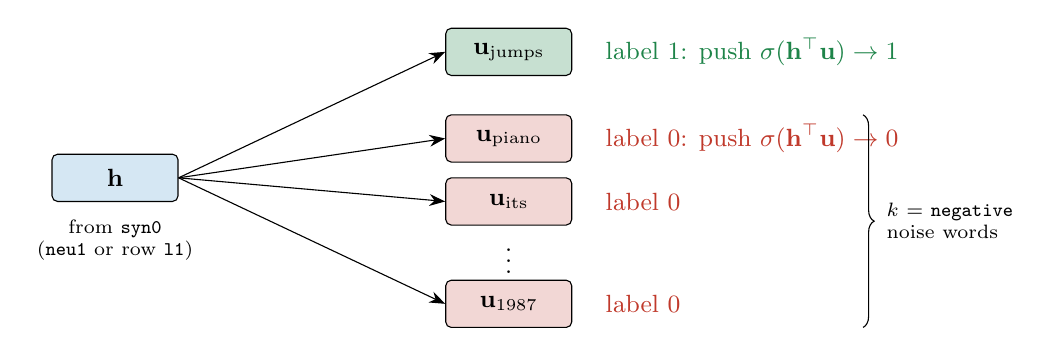
\begin{tikzpicture}[
  vec/.style={draw,rounded corners=2pt,minimum width=16mm,minimum height=6mm,font=\small},
  arr/.style={-{Stealth[length=2mm]}}]
  \node[vec,fill=incol!20] (h) at (0,0) {$\mathbf{h}$};
  \node[font=\scriptsize,below=1mm of h,align=center] {from \code{syn0}\\(\code{neu1} or row \code{l1})};
  \node[vec,fill=poscol!25] (p)  at (5,1.6)  {$\vout_{\text{jumps}}$};
  \node[vec,fill=negcol!20] (n1) at (5,0.5)  {$\vout_{\text{piano}}$};
  \node[vec,fill=negcol!20] (n2) at (5,-0.3) {$\vout_{\text{its}}$};
  \node[font=\small] at (5,-0.95) {$\vdots$};
  \node[vec,fill=negcol!20] (n5) at (5,-1.6) {$\vout_{\text{1987}}$};
  \foreach \n in {p,n1,n2,n5} \draw[arr] (h.east) -- (\n.west);
  \node[right=3mm of p,font=\small,poscol] {label 1: push $\sigma(\mathbf{h}^{\top}\vout)\to 1$};
  \node[right=3mm of n1,font=\small,negcol] {label 0: push $\sigma(\mathbf{h}^{\top}\vout)\to 0$};
  \node[right=3mm of n2,font=\small,negcol] {label 0};
  \node[right=3mm of n5,font=\small,negcol] {label 0};
  \draw[decorate,decoration={brace,amplitude=4pt}] (9.5,0.8) -- (9.5,-1.9)
     node[midway,right=5pt,font=\scriptsize,align=left] {$k$ = \code{negative}\\noise words};
\end{tikzpicture}
\caption{Negative sampling: one positive (the real centre word) and $k$ random
negatives. Only these $k+1$ rows of \code{syn1neg} are touched.}
\label{fig:negsamp}
\end{figure}

\paragraph{The gradient.}
For one term with label $\ell\in\{0,1\}$ and score $x = \mathbf{h}^{\top}\vout$,
the derivative of $\ell\log\sigma(x) + (1-\ell)\log\sigma(-x)$ with respect to $x$ is
simply
\[
  \frac{\partial \mathcal{L}}{\partial x} = \ell - \sigma(x).
\]
This is the whole learning rule. The code calls the step size times this error
\code{g}, then applies the chain rule to both vectors involved:
\[
  g = \alpha\,(\ell - \sigma(x)), \qquad
  \vout \leftarrow \vout + g\,\mathbf{h}, \qquad
  \mathbf{e} \leftarrow \mathbf{e} + g\,\vout .
\]
$\mathbf{e}$ (\code{neu1e}) accumulates the error for the input side. It is applied
to \code{syn0} only after all $k+1$ terms are processed, so every term sees the same
$\mathbf{h}$. Here is the CBOW version:

\begin{lstlisting}[firstnumber=480]
        if (negative > 0) for (d = 0; d < negative + 1; d++) {
          if (d == 0) {
            target = word;              // the real centre word
            label = 1;
          } else {
            next_random = next_random * (unsigned long long)25214903917 + 11;
            target = table[(next_random >> 16) % table_size];   // noise word
            if (target == 0) target = next_random % (vocab_size - 1) + 1;
            if (target == word) continue;
            label = 0;
          }
          l2 = target * layer1_size;
          f = 0;
          for (c = 0; c < layer1_size; c++) f += neu1[c] * syn1neg[c + l2];  // x = h . u
          if (f > MAX_EXP) g = (label - 1) * alpha;
          else if (f < -MAX_EXP) g = (label - 0) * alpha;
          else g = (label - expTable[(int)((f + MAX_EXP) * (EXP_TABLE_SIZE / MAX_EXP / 2))]) * alpha;
          for (c = 0; c < layer1_size; c++) neu1e[c] += g * syn1neg[c + l2];  // e += g u
          for (c = 0; c < layer1_size; c++) syn1neg[c + l2] += g * neu1[c];   // u += g h
        }
\end{lstlisting}

Intuitively: if a real neighbour scores low, $g>0$ pulls $\mathbf{h}$ and
$\vout_o$ together; if a noise word scores high, $g<0$ pushes them apart. Over
millions of updates, words that share neighbours get pulled towards the same
output vectors and so towards each other.

\paragraph{The noise distribution.}
Negatives are drawn from the unigram distribution raised to the power $3/4$:
\[
  P_n(w) = \frac{\code{cn}(w)^{0.75}}{\sum_{w'}\code{cn}(w')^{0.75}} .
\]
The exponent flattens the distribution, so rare words are picked more often than
their raw frequency and common words less. To sample in $O(1)$,
\code{InitUnigramTable()} (\src{58}) fills a table of $10^8$ integers where word
$w$ occupies a share of slots proportional to $P_n(w)$; drawing a uniformly random
slot then samples from $P_n$ (Figure~\ref{fig:table}).

\begin{figure}[ht]
\centering
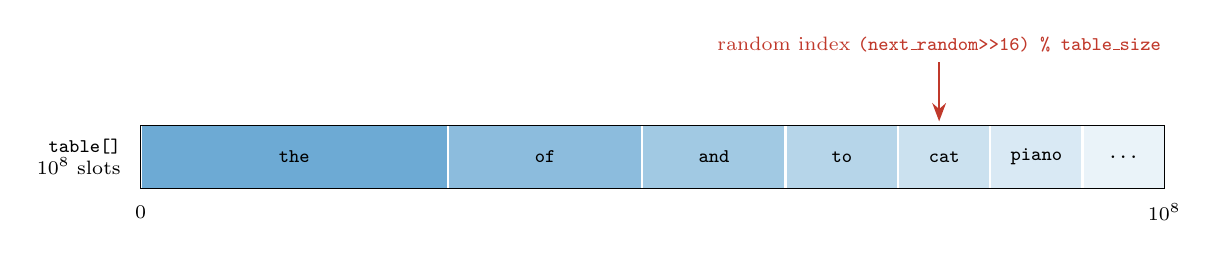
\begin{tikzpicture}[x=1.3mm,y=1mm]
  \foreach \w/\s/\x/\col in {the/30/0/incol!70,of/19/30/incol!55,and/14/49/incol!45,to/11/63/incol!35,cat/9/74/incol!25,piano/9/83/incol!18,\dots/8/92/incol!10} {
    \fill[\col] (\x,0) rectangle ++(\s,8);
    \draw[white,thick] (\x,0) -- ++(0,8);
    \node[font=\scriptsize] at (\x+\s/2,4) {\code{\w}};
  }
  \draw (0,0) rectangle (100,8);
  \node[anchor=east,font=\scriptsize,align=right] at (-1,4) {\code{table[]}\\$10^8$ slots};
  \node[font=\scriptsize] at (0,-3) {0};
  \node[font=\scriptsize] at (100,-3) {$10^8$};
  \draw[-{Stealth},thick,negcol] (78,16) node[above,font=\scriptsize] {random index \code{(next\_random>>16) \% table\_size}} -- (78,8.5);
\end{tikzpicture}
\caption{The unigram table. Each word owns a contiguous run of slots, sized by
$\code{cn}^{0.75}$, so a single random index yields a noise word. Proportions are illustrative.}
\label{fig:table}
\end{figure}

\subsection{Hierarchical softmax (\texttt{-hs 1})}

Hierarchical softmax keeps a true probability distribution over all words but
computes it as a sequence of binary decisions along a path in a binary tree whose
leaves are the words. The probability of a word is the product of the
probabilities of taking each left/right turn on the way from the root to its leaf. Each
inner node $n$ has its own vector $\vout_n$ (a row of \code{syn1}), and the
probability of turning one way at that node is $\sigma(\mathbf{h}^{\top}\vout_n)$.
Only $O(\log V)$ nodes lie on a path.

\paragraph{The Huffman tree.}
\code{CreateBinaryTree()} (\src{214}) builds a \emph{Huffman} tree from the word
counts, so frequent words get short paths and are cheap to train. Because the
vocabulary is already sorted by count, the classic algorithm runs in linear time with
two pointers: \code{pos1} walks left over the leaves (smallest first) and
\code{pos2} walks right over the newly created inner nodes. For each word the
code stores
\begin{itemize}[nosep]
  \item \code{code[]}: the bits ($0$/$1$) of the turns from root to leaf, and
  \item \code{point[]}: the indices of the inner nodes visited, i.e.\ which rows of
        \code{syn1} to use.
\end{itemize}

\begin{figure}[ht]
\centering
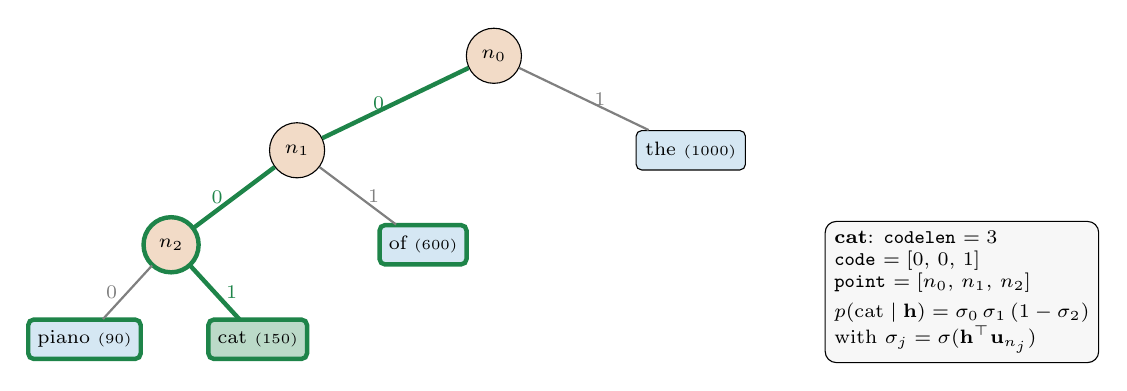
\begin{tikzpicture}[
  level distance=12mm,
  level 1/.style={sibling distance=50mm},
  level 2/.style={sibling distance=32mm},
  level 3/.style={sibling distance=22mm},
  inner/.style={circle,draw,fill=outcol!25,minimum size=7mm,font=\scriptsize},
  leaf/.style={rectangle,rounded corners=2pt,draw,fill=incol!20,font=\scriptsize,minimum height=5mm},
  edge from parent/.style={draw,thick,gray},
  hl/.style={edge from parent/.style={draw,ultra thick,poscol}}]
  \node[inner] {$n_0$}
    child[hl] { node[inner] {$n_1$}
      child[hl] { node[inner] {$n_2$}
        child[edge from parent/.style={draw,thick,gray}] { node[leaf] {piano \tiny(90)}
            edge from parent node[left,font=\scriptsize] {0} }
        child[hl] { node[leaf,fill=poscol!30] {cat \tiny(150)}
            edge from parent node[right,font=\scriptsize] {1} }
        edge from parent node[left,font=\scriptsize] {0} }
      child[edge from parent/.style={draw,thick,gray}] { node[leaf] {of \tiny(600)}
            edge from parent node[right,font=\scriptsize] {1} }
      edge from parent node[left,font=\scriptsize] {0} }
    child[edge from parent/.style={draw,thick,gray}] { node[leaf] {the \tiny(1000)}
            edge from parent node[right,font=\scriptsize] {1} };
  \node[draw,rounded corners,fill=codebg,font=\scriptsize,align=left,anchor=west] at (4.2,-3.0)
    {\textbf{cat}: \code{codelen} $=3$\\
     \code{code}  $= [0,\,0,\,1]$\\
     \code{point} $= [n_0,\,n_1,\,n_2]$\\[3pt]
     $p(\text{cat}\mid\mathbf{h}) = \sigma_0\,\sigma_1\,(1-\sigma_2)$\\
     with $\sigma_j = \sigma(\mathbf{h}^{\top}\vout_{n_j})$};
\end{tikzpicture}
\caption{A toy Huffman tree built as \code{CreateBinaryTree()} does it: repeatedly
merge the two smallest nodes, giving bit 0 to the smaller and 1 to the larger
(\code{binary[min2i] = 1}). The most frequent word sits closest to the root. To
predict \emph{cat}, the model only scores the three inner nodes on the
highlighted path instead of all $V$ words.}
\label{fig:huffman}
\end{figure}

\paragraph{The update.}
At each node on the path the code does one logistic-regression step whose label is
$1-\text{code bit}$. A $0$ bit (turn ``left'') is the positive class:

\begin{lstlisting}[firstnumber=464]
        if (hs) for (d = 0; d < vocab[word].codelen; d++) {
          f = 0;
          l2 = vocab[word].point[d] * layer1_size;   // inner node on the path
          for (c = 0; c < layer1_size; c++) f += neu1[c] * syn1[c + l2];
          if (f <= -MAX_EXP) continue;
          else if (f >= MAX_EXP) continue;
          else f = expTable[(int)((f + MAX_EXP) * (EXP_TABLE_SIZE / MAX_EXP / 2))];
          g = (1 - vocab[word].code[d] - f) * alpha;  // (label - sigma) * alpha
          for (c = 0; c < layer1_size; c++) neu1e[c] += g * syn1[c + l2];
          for (c = 0; c < layer1_size; c++) syn1[c + l2] += g * neu1[c];
        }
\end{lstlisting}

This is the same rule $g=\alpha(\ell-\sigma(x))$ as in negative sampling. The only
difference is where the binary questions come from: tree nodes instead of random
words.

\begin{note}
\textbf{Which one to use?} Hierarchical softmax tends to do better for
infrequent words; negative sampling does better for frequent words and with
low-dimensional vectors. The defaults (\code{-negative 5 -hs 0}) are a good start;
the original README suggests skip-gram with negative sampling for quality and
CBOW for speed.
\end{note}

%======================================================================
\section{Implementation tricks for speed}
%======================================================================

\subsection{The sigmoid lookup table}

Computing \code{exp()} for every update would be slow, so \code{main()} precomputes
$\sigma(x)$ at 1000 points on $[-6,6]$ (\src{739--742}):

\begin{lstlisting}[firstnumber=739]
  for (i = 0; i < EXP_TABLE_SIZE; i++) {
    expTable[i] = exp((i / (real)EXP_TABLE_SIZE * 2 - 1) * MAX_EXP); // Precompute the exp() table
    expTable[i] = expTable[i] / (expTable[i] + 1);                   // Precompute f(x) = x / (x + 1)
  }
\end{lstlisting}

At training time a score $x$ is mapped to the index $\lfloor (x+6)\cdot 83\rfloor$.
Outside $[-6,6]$ the sigmoid is treated as saturated: negative sampling uses
exactly 0 or 1, and hierarchical softmax skips the node. The error is negligible.

\begin{figure}[ht]
\centering
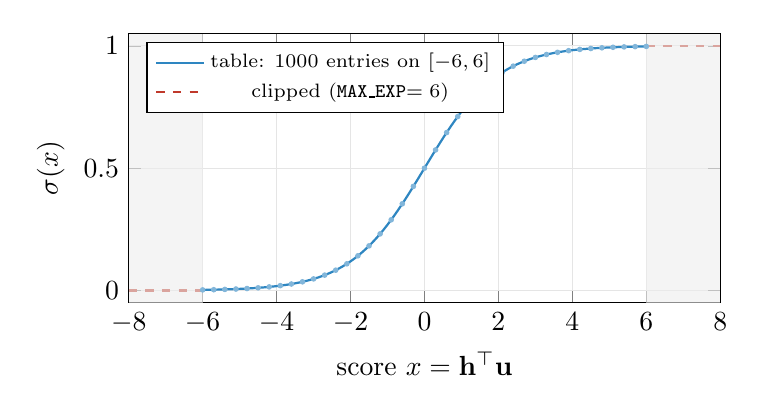
\begin{tikzpicture}
\begin{axis}[
  width=0.75\linewidth,height=5cm,
  xlabel={score $x=\mathbf{h}^{\top}\vout$},ylabel={$\sigma(x)$},
  xmin=-8,xmax=8,ymin=-0.05,ymax=1.05,
  grid=major,grid style={gray!20},
  legend pos=north west,legend style={font=\scriptsize}]
  \addplot[incol,thick,domain=-6:6,samples=200] {1/(1+exp(-x))};
  \addplot[negcol,thick,dashed,domain=-8:-6] {0};
  \addplot[negcol,thick,dashed,domain=6:8,forget plot] {1};
  \addplot[only marks,mark=*,mark size=0.8pt,incol!60,domain=-6:6,samples=41] {1/(1+exp(-x))};
  \legend{{table: 1000 entries on $[-6,6]$},{clipped (\code{MAX\_EXP}$=6$)}}
  \fill[gray!15,opacity=0.6] (axis cs:-8,-0.05) rectangle (axis cs:-6,1.05);
  \fill[gray!15,opacity=0.6] (axis cs:6,-0.05) rectangle (axis cs:8,1.05);
\end{axis}
\end{tikzpicture}
\caption{The sigmoid is read from \code{expTable} inside $[-6,6]$ and treated as 0 or 1
outside it (shaded).}
\end{figure}

\subsection{Learning-rate schedule}

The step size $\alpha$ starts at \code{-alpha} (0.025 for skip-gram, 0.05 for CBOW)
and decreases linearly to almost zero over the whole run. Every 10\,000 words, each
thread recomputes it from the global progress counter:

\begin{lstlisting}[firstnumber=412]
      alpha = starting_alpha * (1 - word_count_actual / (real)(iter * train_words + 1));
      if (alpha < starting_alpha * 0.0001) alpha = starting_alpha * 0.0001;
\end{lstlisting}

Large early steps move the random vectors quickly into a sensible arrangement; small
late steps fine-tune it without jitter.

\begin{figure}[ht]
\centering
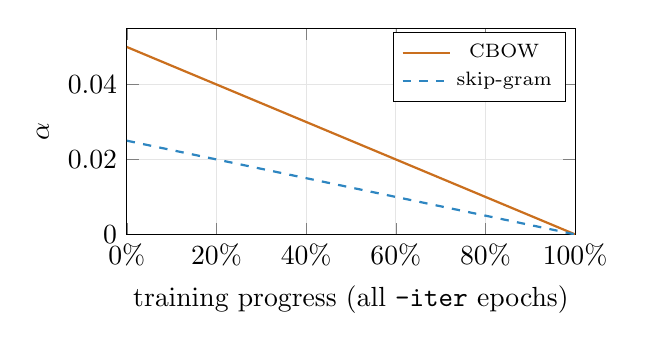
\begin{tikzpicture}
\begin{axis}[
  width=0.6\linewidth,height=4.2cm,
  xlabel={training progress (all \code{-iter} epochs)},ylabel={$\alpha$},
  xmin=0,xmax=1,ymin=0,ymax=0.055,
  xtick={0,0.2,0.4,0.6,0.8,1},xticklabels={0\%,20\%,40\%,60\%,80\%,100\%},
  yticklabel style={/pgf/number format/fixed,/pgf/number format/precision=3},
  scaled y ticks=false,
  grid=major,grid style={gray!20},legend style={font=\scriptsize}]
  \addplot[outcol,thick,domain=0:1] {max(0.05*(1-x),0.05*0.0001)};
  \addplot[incol,thick,dashed,domain=0:1] {max(0.025*(1-x),0.025*0.0001)};
  \legend{CBOW,skip-gram}
\end{axis}
\end{tikzpicture}
\caption{Linear learning-rate decay, floored at $10^{-4}\times$ the starting value.}
\end{figure}

\subsection{Lock-free multithreading (Hogwild)}

\code{TrainModel()} starts \code{-threads} threads. Thread $i$ seeks to byte offset
$i\cdot\code{file\_size}/\code{num\_threads}$ in the training file and processes
$\code{train\_words}/\code{num\_threads}$ words per epoch, repeated for \code{-iter}
epochs (\src{400}, \src{434--443}).

All threads read and write the \emph{same} \code{syn0} and \code{syn1neg} arrays
without any locks. Two threads can occasionally overwrite each other's update to the
same row, but each update touches only a handful of rows out of tens of thousands,
so collisions are rare and the lost updates act like a little extra noise. This
``Hogwild'' style of parallel stochastic gradient descent scales almost linearly
with the number of cores.

\begin{figure}[ht]
\centering
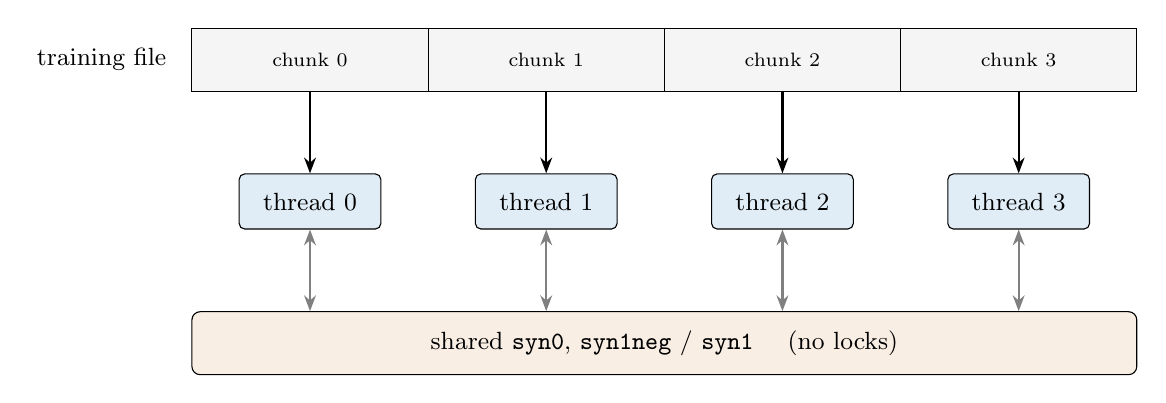
\begin{tikzpicture}[
  th/.style={draw,rounded corners=2pt,fill=incol!15,minimum width=18mm,minimum height=7mm,font=\small},
  arr/.style={{Stealth[length=2mm]}-{Stealth[length=2mm]},thick,gray}]
  \draw[fill=gray!8] (0,0) rectangle (12,0.8);
  \foreach \i in {0,1,2,3} {
    \draw (\i*3,0) -- (\i*3,0.8);
    \node[font=\scriptsize] at (\i*3+1.5,0.4) {chunk \i};
    \node[th] (t\i) at (\i*3+1.5,-1.4) {thread \i};
    \draw[-{Stealth[length=2mm]},thick] (\i*3+1.5,0) -- (t\i);
  }
  \node[anchor=east,font=\small] at (-0.2,0.4) {training file};
  \node[draw,rounded corners=3pt,fill=outcol!12,minimum width=12cm,minimum height=8mm,
        font=\small,align=center] (m) at (6,-3.2) {shared \code{syn0}, \code{syn1neg} / \code{syn1} \quad(no locks)};
  \foreach \i in {0,1,2,3} \draw[arr] (t\i) -- (t\i |- m.north);
\end{tikzpicture}
\caption{Each thread trains on its own slice of the file, while all threads update
the shared weight matrices concurrently.}
\end{figure}

%======================================================================
\section{Putting it together: one training step}
%======================================================================

Figure~\ref{alg:step} condenses \code{TrainModelThread()} for skip-gram with
negative sampling (the CBOW path differs only in averaging the context first).

\begin{figure}[ht]
\centering
\fbox{\begin{minipage}{0.92\linewidth}
\small
\textbf{for} each epoch, \textbf{for} each sentence in this thread's chunk:\\[2pt]
\hspace*{1em}read words up to \code{</s>}; drop each occurrence of $w$ with probability $1-P_{\text{keep}}(w)$\\
\hspace*{1em}\textbf{for} each position $p$ with centre word $o$:\\
\hspace*{2em}$b \leftarrow$ random in $[0,\code{window})$\\
\hspace*{2em}\textbf{for} each context word $c$ within $\code{window}-b$ of $p$:\\
\hspace*{3em}$\mathbf{e}\leftarrow \mathbf{0}$\\
\hspace*{3em}\textbf{for} $(t,\ell)$ in $\{(o,1)\}\cup\{(n_i,0)\}_{i=1}^{k}$, \quad $n_i\sim P_n$:\\
\hspace*{4em}$x \leftarrow \vin_c^{\top}\vout_t$;\quad $g \leftarrow \alpha(\ell-\sigma(x))$\\
\hspace*{4em}$\mathbf{e} \leftarrow \mathbf{e} + g\,\vout_t$;\quad $\vout_t \leftarrow \vout_t + g\,\vin_c$\\
\hspace*{3em}$\vin_c \leftarrow \vin_c + \mathbf{e}$\\
\hspace*{1em}every 10\,000 words: $\alpha \leftarrow \alpha_0\max\!\big(1-\text{progress},\,10^{-4}\big)$
\end{minipage}}
\caption{One thread's training loop (skip-gram, negative sampling).}
\label{alg:step}
\end{figure}

%======================================================================
\section{Step 5: the output and how it is used}
%======================================================================

\subsection{The vector file}

After all threads finish, \code{TrainModel()} writes \code{syn0}, the input
vectors. The first line is ``$V$ $d$''. Each following line holds a word and its $d$
components, as text or, with \code{-binary 1}, as raw 4-byte floats
(\src{593--601}). The output matrices are discarded.

With \code{-classes K}, the program instead runs 10 iterations of $k$-means on the
vectors (using normalised centroids and dot-product similarity) and writes one
``word cluster-id'' line per word (\src{602--645}).

\subsection{Querying the vectors}

All query tools load the file, normalise each vector to unit length, and compare
vectors by \emph{cosine similarity}:
\[
  \cos(\mathbf{a},\mathbf{b}) = \frac{\mathbf{a}^{\top}\mathbf{b}}{\lVert\mathbf{a}\rVert\,\lVert\mathbf{b}\rVert}
  \in[-1,1].
\]

\begin{center}
\begin{tabularx}{\linewidth}{@{}lX@{}}
\toprule
Program & What it does \\
\midrule
\code{distance} & Reads one or more words, averages and normalises their vectors, and
prints the 40 vocabulary words with the highest cosine similarity (excluding the
query words). \\
\code{word-analogy} & Reads three words $a\;b\;c$, computes $\vin_b-\vin_a+\vin_c$, and
prints the 40 nearest words, e.g.\ \emph{paris france berlin} $\to$ \emph{germany}. \\
\code{compute-accuracy} & Runs the analogy questions in \code{questions-words.txt}
(``\emph{athens greece baghdad iraq}''), restricted to the most frequent words
(e.g.\ 30\,000), and reports top-1 accuracy split into semantic and syntactic sections. \\
\bottomrule
\end{tabularx}
\end{center}

\subsection{Phrases: \texttt{word2phrase}}

Some meanings belong to multi-word units: \emph{new york}, \emph{air canada}.
\code{word2phrase} makes one pass over the corpus counting unigrams and bigrams, then
joins a bigram $ab$ into a single token \code{a\_b} when
\[
  \text{score}(a,b) = \frac{\code{cn}(ab) - \code{min\_count}}{\code{cn}(a)\cdot\code{cn}(b)}\cdot \code{train\_words} \;>\; \code{threshold}
  \quad(\text{default }100).
\]
The score is high when $a$ and $b$ occur together far more often than chance would
predict. Subtracting \code{min\_count} stops rare coincidences from becoming phrases.
Running it twice builds phrases of up to four words, as \code{demo-phrases.sh} does,
and \code{word2vec} then learns vectors for the phrase tokens like any other word.

%======================================================================
\section{Hyperparameters at a glance}
%======================================================================

\begin{center}
\small
\begin{tabularx}{\linewidth}{@{}llX@{}}
\toprule
Option & Default & Effect \\
\midrule
\code{-size} & 100 & Vector dimension $d$. Larger captures more but needs more data. \\
\code{-window} & 5 & Maximum context reach. Small windows favour syntactic similarity, large ones topical similarity. \\
\code{-cbow} & 1 & 1 = CBOW (fast), 0 = skip-gram (slower, better for rare words). \\
\code{-negative} & 5 & Noise words per positive example; 0 disables negative sampling. \\
\code{-hs} & 0 & 1 enables hierarchical softmax. \\
\code{-sample} & $10^{-3}$ & Subsampling threshold $t$; smaller drops more frequent words. \\
\code{-alpha} & 0.05 / 0.025 & Starting learning rate (CBOW / skip-gram). \\
\code{-iter} & 5 & Number of passes over the corpus. \\
\code{-min-count} & 5 & Discard words rarer than this. \\
\code{-threads} & 12 & Parallel training threads. \\
\code{-binary} & 0 & Write vectors as binary floats instead of text. \\
\code{-classes} & 0 & If $>0$, output $k$-means cluster ids instead of vectors. \\
\bottomrule
\end{tabularx}
\end{center}

A typical high-quality run on \code{text8}, as in the README:
\begin{lstlisting}[language=bash,numbers=none,morekeywords={}]
./word2vec -train text8 -output vectors.bin -cbow 1 -size 200 -window 8 \
           -negative 25 -hs 0 -sample 1e-4 -threads 8 -binary 1 -iter 15
\end{lstlisting}

%======================================================================
\section*{Appendix: code map}
\addcontentsline{toc}{section}{Appendix: code map}
%======================================================================

\begin{center}
\small
\begin{tabularx}{\linewidth}{@{}llX@{}}
\toprule
Function & Lines & Role \\
\midrule
\code{InitUnigramTable} & 58--74 & Builds the $\code{cn}^{0.75}$ noise table for negative sampling. \\
\code{ReadWord} & 77--101 & Tokeniser; newline becomes \code{</s>}. \\
\code{GetWordHash}, \code{SearchVocab} & 104--120 & Hash-table lookup with linear probing. \\
\code{AddWordToVocab} & 134--150 & Inserts a new word, growing the array as needed. \\
\code{SortVocab} & 161--188 & Sort by count, drop rare words, allocate Huffman arrays. \\
\code{ReduceVocab} & 191--210 & Prunes the vocabulary when the hash table fills up. \\
\code{CreateBinaryTree} & 214--277 & Linear-time Huffman tree; fills \code{code} and \code{point}. \\
\code{LearnVocabFromTrainFile} & 279--315 & First pass over the corpus: counts words. \\
\code{InitNet} & 361--383 & Allocates and initialises \code{syn0}, \code{syn1}, \code{syn1neg}. \\
\code{TrainModelThread} & 385--570 & The training loop: subsampling, window, CBOW/skip-gram, HS/NS updates. \\
\code{TrainModel} & 572--647 & Orchestrates everything; writes vectors or $k$-means classes. \\
\code{main} & 670--745 & Parses options, precomputes \code{expTable}. \\
\bottomrule
\end{tabularx}
\end{center}

\section*{Further reading}
\addcontentsline{toc}{section}{Further reading}
\begin{itemize}[nosep]
  \item T.~Mikolov, K.~Chen, G.~Corrado, J.~Dean. \emph{Efficient Estimation of Word
        Representations in Vector Space}. ICLR Workshop, 2013.
  \item T.~Mikolov, I.~Sutskever, K.~Chen, G.~Corrado, J.~Dean. \emph{Distributed
        Representations of Words and Phrases and their Compositionality}. NeurIPS, 2013.
  \item Y.~Goldberg, O.~Levy. \emph{word2vec Explained: Deriving Mikolov et al.'s
        Negative-Sampling Word-Embedding Method}. arXiv:1402.3722, 2014.
  \item \code{ARCHITECTURE.md} and \code{BUILD\_AND\_USAGE.md} in this repository.
\end{itemize}

\end{document}
